\chapter{1893 Issue} 

The change in the colour of the Turks Islands Twopence halfpenny
was suggested by De La Rue when the first requisition since the
approval of the Postal Union colour scheme was received on July 5,1892:

\begin{quotation}
There is little confusion in this requisition as it stated that
the stamps are required to be printed in the same colour as the last
issue, viz. that of the Postal Union. The last lot of stamps printed
were in copper red, whereas the Postal Union colour is blue. With
your consent, we would propose therefore to print this supply in blue,
the more so as the 2 1/2 d. was printed in blue on the colour scheme 
submitted by us on the 25th September 1883, which scheme was
subsequently approved by the Colonial letter of the 23rd January 1884.

\end{quotation}

\begin{marginfigure}
\centering
\rule{0cm}{21.3cm}
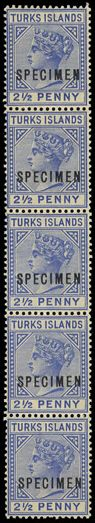
\includegraphics[width=.60\textwidth]{../turks-islands/2389.jpg}
\caption{2389
SP
\#43 (SG65) 1893 QV 2 1/2d ultramarine vertical strip of 5 from column 6, 
overprinted Specimen. Scarce in this format as De la Rue supplied 10 
horizontal strips and just 2 vertical ones. NH. F-VF. 
(as singles SG \pound250). 
PHOTO
\$  160 }
\end{marginfigure}

Lorem ipsum dolor sit amet, consectetur adipiscing elit. Sed nibh justo, dictum sed cursus ac, lobortis et lacus. Vestibulum vitae justo enim. Quisque laoreet elementum felis, ut sodales arcu viverra a. Sed molestie odio vulputate sem rutrum a sagittis est rutrum. Morbi dapibus hendrerit magna, sit amet commodo massa posuere sit amet. Duis pharetra quam scelerisque est lobortis fringilla. Maecenas venenatis feugiat lectus, vel facilisis odio pharetra quis. Etiam at nisl eros, sit amet suscipit lorem. Lorem ipsum dolor sit amet, consectetur adipiscing elit. Sed augue nunc, ornare eget congue sit amet, laoreet vel augue. Morbi vel justo quis ipsum adipiscing egestas vitae non est. Vivamus ac quam quam. Nullam pharetra
                                                    interdum mauris, rutrum pulvinar ligula condimentum id. Donec et blandit lorem. Lorem ipsum dolor sit amet, consectetur adipiscing elit. Sed nibh justo, dictum sed cursus ac, lobortis et lacus. Vestibulum vitae justo enim. Quisque laoreet elementum felis, ut sodales arcu viverra a. Sed molestie odio vulputate sem rutrum a sagittis est rutrum. Morbi dapibus hendrerit magna, sit amet commodo massa posuere sit amet. Duis pharetra quam scelerisque est lobortis fringilla. Maecenas venenatis feugiat lectus, vel facilisis odio pharetra quis. Etiam at nisl eros, sit amet suscipit lorem. Lorem ipsum dolor sit amet, consectetur adipiscing elit. Sed augue nunc, ornare eget congue sit amet, laoreet vel augue. Morbi vel justo quis ipsum adipiscing egestas vitae non est. Vivamus ac quam quam. Nullam pharetra
                                                    interdum mauris, rutrum pulvinar ligula condimentum id. Donec et blandit lorem. 

\ph[width=.98\textwidth]{../turks-islands/2390.jpg}{2390
SP
\#43 (SG65) 1893 QV 2 1/2d ultramarine horizontal strip of 5 overprinted 
Specimen, the right stamp, variety broken 'M' in 'Specimen', pos. 41. 
NH. F-VF. (as singles SG \pound250). PHOTO
\$  190}

Lorem ipsum dolor sit amet, consectetur adipiscing elit. Sed nibh justo, dictum sed cursus ac, lobortis et lacus. Vestibulum vitae justo enim. Quisque laoreet elementum felis, ut sodales arcu viverra a. Sed molestie odio vulputate sem rutrum a sagittis est rutrum. Morbi dapibus hendrerit magna, sit amet commodo massa posuere sit amet. Duis pharetra quam scelerisque est lobortis fringilla. Maecenas venenatis feugiat lectus, vel facilisis odio pharetra quis. Etiam at nisl eros, sit amet suscipit lorem. Lorem ipsum dolor sit amet, consectetur adipiscing elit. Sed augue nunc, ornare eget congue sit amet, laoreet vel augue. Morbi vel justo quis ipsum adipiscing egestas vitae non est. Vivamus ac quam quam. Nullam pharetra
                                                    interdum mauris, rutrum pulvinar ligula condimentum id. Donec et blandit lorem. Lorem ipsum dolor sit amet, consectetur adipiscing elit. Sed nibh justo, dictum sed cursus ac, lobortis et lacus. Vestibulum vitae justo enim. Quisque laoreet elementum felis, ut sodales arcu viverra a. Sed molestie odio vulputate sem rutrum a sagittis est rutrum. Morbi dapibus hendrerit magna, sit amet commodo massa posuere sit amet. Duis pharetra quam scelerisque est lobortis fringilla. Maecenas venenatis feugiat lectus, vel facilisis odio pharetra quis. Etiam at nisl eros, sit amet suscipit lorem. Lorem ipsum dolor sit amet, consectetur adipiscing elit. Sed augue nunc, ornare eget congue sit amet, laoreet vel augue. Morbi vel justo quis ipsum adipiscing egestas vitae non est. Vivamus ac quam quam. Nullam pharetra
                                                    interdum mauris, rutrum pulvinar ligula condimentum id. Donec et blandit lorem. 




\ph[width=.20\textwidth]{../turks-islands/2391.jpg}{
2391
\#43var (SG50w) 1881 QV 4d ultramarine wmk Crown CC, variety watermark 
inverted, used. This stamp is the discovery copy and forms the basis 
for the SG listing. Small facial scrape at bottom. Fine. (SG \pound375). 
\$ 160
}

\ph[width=.40\textwidth]{../turks-islands/2392.jpg}{
2392
\#44 (SG55) 1883 QV 1d orange-brown bottom margin block of 4 
wmk Crown CA reversed. OG. An exceptional block. Thin in margin. 
F-VF+. Ex Ludington and Baillie. (Scott \$310, SG \pound400). PHOTO
\$  250
}

\ph[width=.20\textwidth]{../turks-islands/2393.jpg}{
2393
SP
\#46 (SG59s) 1889 QV 6d yellow-brown wmk Crown CA 
perf 14 vertical pair overprinted Specimen. NH. F-VF. (SG \pound100). PHOTO
\$ 60
}


\ph[width=.98\textwidth]{../turks-islands/2395.jpg}{
2395
1890 QV 4d grey on registered cover to London cancelled TI and with 
oval REGISTERED DE 30 89 alongside. "R" in oval and Liverpool 
transit at UL. Red reg. London arrival below. Very attractive. PHOTO
\$ 200
}

\ph[width=.98\textwidth]{../turks-islands/2396.jpg}{
2396
1893 QV 2 1/2d red-brown on cover to Beckenham cancelled TI and with 
TURKS ISLANDS FE 25 93 cds alongside. F-VF. PHOTO
\$ 170
}


\ph[width=.98\textwidth]{../turks-islands/2398.jpg}{2390
2398
1897 QV 1/2d (4) and 2\half d (2) on registered letter to the Bahamas, 
the stamps cancelled light TI and with oval REGISTERED FE 5 97 alongside. 
At UL red "A.R.". Bs Nassau, New Providence MR 1. Cover seriously torn 
but affecting one stamp only. Fine. PHOTO
\$ 120
}

\ph[width=.60\textwidth]{../turks-islands/2399.jpg}{2390
2399
\#55, variety (SG61, variety) 1889 QV 1d on 2 1/2d red-brown horizontal strip of 3, 
two stamps, variety overprint misplaced diagonally, used. 
Center stamp with only the "e" of "One" visible. A striking error. 
Light crayon line at bottom and one or 2 short perfs. F-VF. Ex Ludington. PHOTO
\$ 400
}
\ph[width=.40\textwidth]{../turks-islands/2400.jpg}{2400
\#55d (SG61b) 1889 QV 1d on 2 1/2d red-brown vertical bisect on small piece 
cancelled bold TI. F-VF. (on cover Scott \$5,500, SG \pound5,000). PHOTO
\$ 400 }

\ph[width=.98\textwidth]{../turks-islands/2401.jpg}{2401
1891 QV 1d on 2 1/2d red-brown (SG61) on cover front to Saxony bearing bottom 
margin horizontal strip of 5 with control number 1 twice, plus single 
stamp all cancelled TI and with TURKS ISLANDS MY 26 91 cds alongside. Very attractive. PHOTO
\$ 100 }

\ph[width=.98\textwidth]{../turks-islands/2402.jpg}{2402
1902 QV 1d on 2\half d red-brown (SG61) and 4d grey (SG57) on registered cover 
to Berlin each stamp cancelled TI and with oval registered ds of MY 1 02 alongside. 
Liverpool and London transits and German arrival on reverse. F-VF. PHOTO
\$ 120. }

\ph[width=.98\textwidth]{../turks-islands/2403.jpg}{2403
1893 QV \half d on 4d grey, setting 2 (SG67), on cover to Bermuda paying the \half d 
printed matter rate, cancelled TI. Ms Recd. 4 July 1893. F-VF. PHOTO
\$ 450 }                  

\ph[width=.40\textwidth]{../turks-islands/2404.jpg}{
2404
\#45, 52-3, 55, 57 (SG61, 63, 65, 71-2) 1889//94 QV group of 5 used blocks with 
1d on 2\half d red-brown, 1d lake, 2\half d ultramarine, 4d dull purple and 
ultramarine 
and 5d olive-green and carmine. All fresh and F-VF. The 5d block ex Ludington. 
(Scott \$204, SG \pound266). 
\$ 140
}

\ph[width=.20\textwidth]{../turks-islands/2405.jpg}{2405
SP
\#53, 57 (SG71s-72s) 1894-95 QV 4d dull purple and ultramarine and 5d 
olive-green and carmine each overprinted Specimen. OG, HR. F-VF. 
(SG \pound100). PHOTO
\$ 60 }

\ph[width=.20\textwidth]{../turks-islands/2406.jpg}{2406
SP
\#57 (SG72s) 1894 QV 5d olive-green and carmine overprinted Specimen, 
variety broken "M" in "Specimen", pos. 41. OG, HR. F-VF. (SG \pound50++). PHOTO
\$ 80}



















                                              